
\begin{frame}{AS7007}
{\fontsize{8}{9}\selectfont\url{https://seclists.org/nanog/1997/Apr/444}}

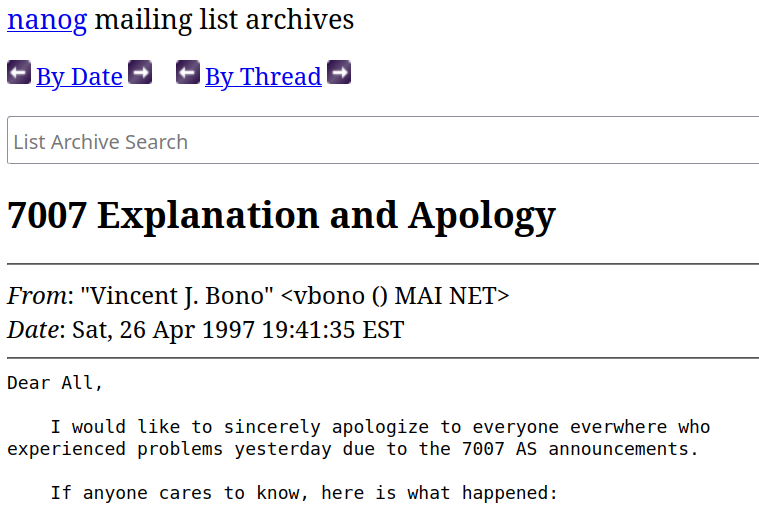
\includegraphics[width=0.4\textwidth]{../routing/as7007-1.png}
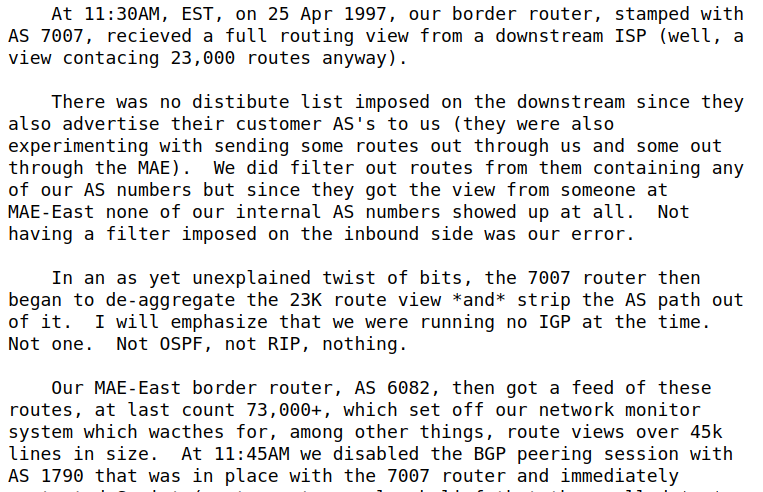
\includegraphics[height=0.4\textwidth]{../routing/as7007-2.png}
\end{frame}

\begin{frame}{2008 Pakistan Youtube}
\begin{itemize}
\item Pakistan Telecom recieved gov't order to block youtube
\item implemented by inserting route for YouTube's IP in internal network
\vspace{.5cm}
\item misconfiguration meant route was advertised on BGP
\item was more specific than YouTube's route, so made YouTube unreachablej
\end{itemize}
\end{frame}

\begin{frame}{timeline from RIPE NCC}
\begin{itemize}
\item {\tiny \url{https://www.ripe.net/about-us/news/youtube-hijacking-a-ripe-ncc-ris-case-study/}}
\item Youtube is announcing 208.65.152.0/22
\item 18:47Z: Pakistan Telecom starts announcing 208.65.153.0/24
\item 20:07Z: Youtube starts announcing 208.65.153.0/24
\item 20:18Z: Youtube starts announcing 208.65.153.0/25 and 208.65.153.128/25
\item 20:51Z: Pakistan Telecom's ISP forwards their announcements with additional copy of Pakistan Telecom's AS number
\item 21:01Z: Pakistan Telecom's ISP withdraws routes initiated by Pakistan Telecom (but not Pakistan Telecom's customers)
\end{itemize}
\end{frame}

\begin{frame}{BGP Hijacking targeted cryptocurrency stuff}
    \begin{itemize}
    \item KLAYswap (Feb 2022), Celer Bridge (Sep 2022)
    \item attackers intentionally redirected traffic to malicious version of services
    \item \ldots and stole money
    \vspace{.5cm}
    \item both probably spoofed the final AS number in AS path
    \item sometimes involved adding attacked IP range to routing registry
    \end{itemize}
\end{frame}

\begin{frame}{nation-states?}
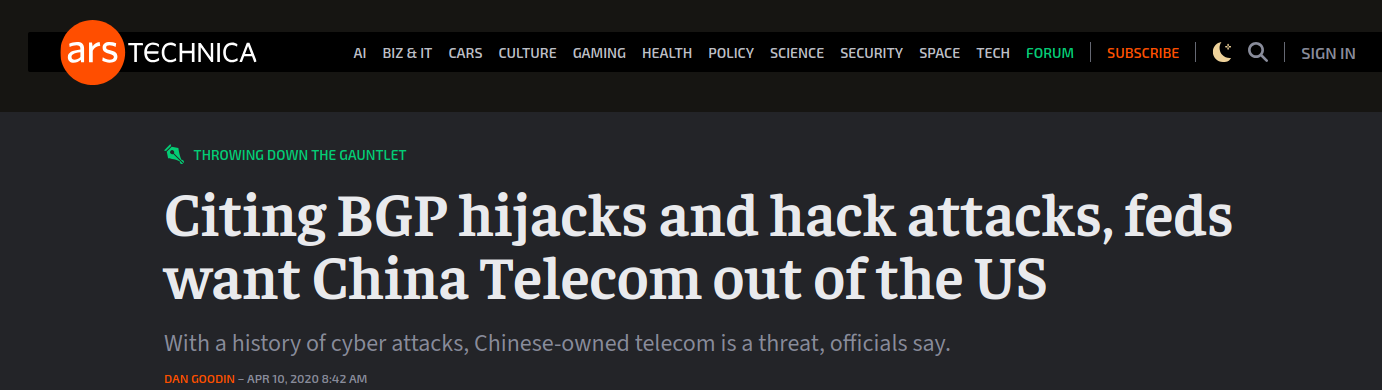
\includegraphics[width=\textwidth]{../routing/china-tele-ars-tech}
\end{frame}
